%% 
%% Copyright 2007-2024 Elsevier Ltd
%% 
%% This file is part of the 'Elsarticle Bundle'.
%% ---------------------------------------------
%%  
%% It may be distributed under the conditions of the LaTeX Project Public
%% License, either version 1.3 of this license or (at your option) any%% later version.  The latest version of this license is in
%%    http://www.latex-project.org/lppl.txt
%% and version 1.3 or later is part of all distributions of LaTeX
%% version 1999/12/01 or later.
%% 
%% The list of all files belonging to the 'Elsarticle Bundle' is
 %% given in the file `manifest.txt'.
%% 
%% Template article for Elsevier's document class `elsarticle'
%% with harvard style bibliographic references

\documentclass[preprint,12pt,authoryear]{elsarticle}

%% Use the option review to obtain double line spacing
%% \documentclass[authoryear,preprint,review,12pt]{elsarticle}

%% Use the options 1p,twocolumn; 3p; 3p,twocolumn; 5p; or 5p,twocolumn
 %% for a journal layout:
%% \documentclass[final,1p,times,authoryear]{elsarticle}
%% \documentclass[final,1p,times,twocolumn,authoryear]{elsarticle}
%% \documentclass[final,3p,times,authoryear]{elsarticle}
%% \documentclass[final,3p,times,twocolumn,authoryear]{elsarticle}
%% \documentclass[final,5p,times,authoryear]{elsarticle}
%% \documentclass[final,5p,times,twocolumn,authoryear]{elsarticle}

%% For including figures, graphicx.sty has been loaded in
%% elsarticle.cls. If you prefer to use the old commands
%% please give \usepackage{epsfig}

%% The amssymb package provides various useful mathematical symbols
\usepackage{amssymb}
\usepackage{graphicx}
%% The amsmath package provides various useful equation environments.
\usepackage{amsmath}
\usepackage{algorithm}
\usepackage{algorithmicx}
\usepackage{algpseudocode}
%% The amsthm package provides extended theorem environments
%% \usepackage{amsthm}

%% The lineno packages adds line numbers. Start line numbering with
%% \begin{linenumbers}, end it with \end{linenumbers}. Or switch it on
%% for the whole article with \linenumbers.
%% \usepackage{lineno}

\journal{Computers and Operation Research}

\begin{document}

\begin{frontmatter}

%% Title, authors and addresses

%% use the tnoteref command within \title for footnotes;
%% use the tnotetext command for theassociated footnote;
%% use the fnref command within \author or \affiliation for footnotes;
%% use the fntext command for theassociated footnote;
%% use the corref command within \author for corresponding author footnotes;
%% use the cortext command for theassociated footnote;
%% use the ead command for the email address,
%% and the form \ead[url] for the home page:
%% \title{Title\tnoteref{label1}}
%% \tnotetext[label1]{}
%% \author{Name\corref{cor1}\fnref{label2}}
%% \ead{email address}
%% \ead[url]{home page}
%% \fntext[label2]{}
%% \cortext[cor1]{}
%% \affiliation{organization={},
%%            addressline={}, 
%%            city={},
%%            postcode={}, 
%%            state={},
%%            country={}}
%% \fntext[label3]{}

\title{Actor-based Large Neighborhood Search} %% Article title

%% use optional labels to link authors explicitly to addresses:
%% \author[label1,label2]{}
%% \affiliation[label1]{organization={},
%%             addressline={},
%%             city={},
%%             postcode={},
%%             state={},
%%             country={}}
%%
%% \affiliation[label2]{organization={},
%%             addressline={},
%%             city={},
%%             postcode={},
%%             state={},
%%             country={}}

\author{Christian Brunbjerg Jespersen} %% Author name
\author{Thomas Jacob Riis Stidsen}
\author{Kristoffer Sigsgaard Wernblad}

%% Author affiliation
\affiliation{organization={Technical University of Denmark},%Department and Organization
            addressline={Anker Egelundsvej 1}, 
            city={Kongens Lyngby},
            postcode={2800}, 
            state={Hovedstaden},
            country={Denmark}}
\affiliation{organization={Technical University of Denmark},%Department and Organization
            addressline={Anker Egelundsvej 1}, 
            city={Kongens Lyngby},
            postcode={2800}, 
            state={Hovedstaden},
            country={Denmark}}
\affiliation{organization={Technical University of Denmark},%Department and Organization
            addressline={Anker Egelundsvej 1}, 
            city={Kongens Lyngby},
            postcode={2800}, 
            state={Hovedstaden},
            country={Denmark}}

%% Abstract
\begin{abstract}
%% Text of abstract
Serveral problems facing the operations research field have proven difficult to solve due to their inherrent uncertainty
and highly dynamic nature. Stochastic optimization, fuzzy logic, and robust optimization are some of the methods that 
have been proposed to solve these issues. These methods make an implicit assumption on static data and
a static problem setting. This paper will argue that a new class of optimization methods will have to be developed by
reflect the need optimizing in a settings where: the data source is changing in real-time; where external inputs affects
the optimization process; where multiple actors are making interdependent decision whose objectives may differ significantly.
This paper proposes an actor-based implementation of the classic large neighborhood search metaheuristic as a specific 
contribution to optimization approachs that more naturally model the dynamic nature of many operational problems.
\end{abstract}

%%Graphical abstract
\begin{graphicalabstract}
%\includegraphics{grabs}
\end{graphicalabstract}

%%Research highlights
\begin{highlights}
\item How to allow direct and real-time integration into an optimization process?
\item How to perform optimmization in a real-time changing parameter space?
\end{highlights}

%% Keywords
\begin{keyword}
%% keywords here, in the form: keyword \sep keyword
Large Neighborhood Search \sep Actor Framework \sep Real-time Optimization \sep Human-centered Computing \sep Interactive Systems and Tools \sep Decision Support Systems \sep Interactive Optimization.


%% PACS codes here, in the form: \PACS code \sep code

%% MSC codes here, in the form: \MSC code \sep code
%% or \MSC[2008] code \sep code (2000 is the default)

\end{keyword}

\end{frontmatter}

%% Add \usepackage{lineno} before \begin{document} and uncomment 
%% following line to enable line numbers
%% \linenumbers

%% main text
%%

%% Use \section commands to start a section
\section{Introduction}
\label{sec:1-introduction}
%% Labels are used to cross-reference an item using \ref command.

Dynamic and operational problems have proven hard to solve in operation research due to the need of tight integration with tacit knowledge of decision makers, as clearly demonstrated by (\citep{barthelemy_human_2002}).
Solving operation research problems that are highly operational in nature have three additional requirements over conventional static solution approaches: they have to be responsive to changing parameters; 
able to be assimilated into the decision makers workflow; allow for integration with dynamic data sources such as databases and RESTapi \citep{meignan_review_2015}. 
Operational aspects of operation research, as opposed to higher level strategic and tactical aspects, are characterized by extensive amounts negotiation and feedback on 
proposed solutions (!!!). The lack of integration and responsiveness can lead to solutions that are not directly implemented in practice but instead provides intial suggestions \cite{meignan_review_2015}, which are
then iterated on later manually. In \citep{barthelemy_human_2002} the authors argue that many problems that operation research aim to solve often in reality comprised of group of individual whose decisions are 
aggregated into an "epistemic subject" on which a mathematical model to proposed and solved, with the VRP being one example. Furthermore some multi-objective optimization problems are a product of 
there being multiple actors in the decision making process each with different views on an optimal solution from their vantage point.

This paper proposes a solution method that will allow for real-time optimization based on user-interaction and connection to a dynamic 
data source (changes to the parameter space). The proposed solution method will be tested on the multi-compartment multi-knapsack problem (MCMKP) on a large dataset. 
The large neighborhood search metaheuristic has been chosen due to its properties of naturally being able to work with and fix infeasible solutions and its state of the 
art performance on scheduling and routing problems. 

The paper is divided into four different sections. Section \ref{sec:2-solution-method} explains the model and method in detail that form the fundation of the paper. 
Section \ref{sec:3-results} shows that results coming from the implemented system where the system will be affected by simulated user-interaction. Section \ref{sec:4-discussion} 
will discuss the implications of the research and possible future research directions.

\subsection{The Multi-compartment Multi-knapsack Problem with capacity penalties}
\label{sub1sec2}
The actor-based large neighborhood search is implemented on the MCMKP. The MCMKP was chosen due to its simplicity
while also being sufficiently computationally hard to illustrate the principle behind the Actor-based LNS. The model is comprised of 
five different sets. $K$ is the number of knapsacks; $I$ is the number of items; $C$ is the number of compartments; $Q$ is a set that
defines which items should be excluded from a specific knapsack; $P$ is an inclusion set that defines the allocation of specific item sets 
which should be included in a specific knapsack. The model has four parameters. $v_{ik}$ is the value of item i in knapsack k; $d$ is the 
penalty for exceeding compartment capacity; $w_{ic}$ is the capacity requirement for item i in compartment c; $cap_{kc}$ is the total amount 
of capacity available in knapsack k for compartment c. The model has 2 decision variables. $x_{ik}$, is a binary decision variable equal to one 
if item i is in knapsack k and zero otherwise; $p_{kc}$ is non-negative decision variable equal to the amount of excess capacity above 
the $c_{kc}$ in knapsack k for compartment c. The parameters $v$, $cap$, $Q$, and $P$ are functions of time, $t$, in this case as they will be 
subject to change during the solution process.

\begin{alignat}{2}
	& \text{Min} \quad \sum_{i = 1}^{I} \sum_{k = 1}^{K} v_{ik}(t) \cdot x_{ik}(t) + \sum_{k = 1}^{K} \sum_{c = 1}^C d \cdot p_{kc}(t)   \label{eqn:objective_function_strategic} \\[1em]
    & \text{subject to:} \notag                                                                                                                                        \\[1em]
	& \sum_{i=1}^I w_{ic} \cdot x_{ik}(t) \leq \ cap_{kc}(t) + p_{kc}(t)        && \forall k \in K, \forall c \in C                      \label{eqn:capacity_constraint}          \\[1em]
	& \sum_{i = 1}^{I} x_{ik}(t) = 1                                            && \forall k \in K                                       \label{eqn:single_workorder_constraint}  \\[1em]
	& x_{ik}(t) = 0                                                             && \forall (i, k) \in Q(t)                               \label{eqn:exclusion_constraint}         \\[1em]
	& x_{ik}(t) = 1                                                             && \forall (i, k) \in P(t)                               \label{eqn:inclusion_constraint}         \\[1em]
	& x_{ik}(t) \in \{0, 1\}                                                    && \forall i \in I, \forall k \in K                      \label{eqn:x_integrality_constraint}     \\[1em] 
	& p_{kc}(t) \in \mathbb{R}^{+}                                              && \forall k \in K, \forall c \in C                      \label{eqn:p_non_negativity_constraint}
\end{alignat}

The objective function \ref{eqn:objective_function_strategic} minimizes the total weight of all item set assignments together with the penalty $d$ for exceeding the 
capacity given in constraint \ref{eqn:capacity_constraint}. Constraint \ref{eqn:capacity_constraint} ensures that all the weights $w_{ic}$ for each item in an item set, given that it
has been assigned, is lower than the capacity for each knapsack k and for each compartment $c$. $p_{kc}$ is the amount of exceeded capacity that is needed for the current assignment of item sets to be feasible.
Constraint \ref{eqn:single_workorder_constraint} makes sure that each item set is assigned to atleast a single knapsack. Constraint \ref{eqn:exclusion_constraint} excludes item sets from 
certain knapsacks and constraint \ref{eqn:inclusion_constraint}  forces a specific item set to be in a specific knapsack. Constraint \ref{eqn:x_integrality_constraint} and \ref{eqn:p_non_negativity_constraint} 
specify the variable domain for $x_{ik}$ and $p_{kc}$ respectively. The effects of changing $Q$, $P$, $cap$, and $v$ in real-time will be examined to determine their effects on the solution and objective value.

\section{Solution Method}
\label{sec:2-solution-method}

\subsection{Actor-based Large Neighborhood Search}
A problem that is affected by user-interaction and requires real-time feedback you need an optimization approach that is able to repair infeasible solutions and while also 
converging quickly. For this the large neighborhood search metaheuristic has been shown satisfy these requirements in the literature \cite{gendreau_handbook_2019}. 

The LNS metaheuristic is defined for static problems, meaning that the parameters that make up the problem instance is not subject to change 
after the algorithm has been started. To make the LNS able adapt to changing parameters in real-time a message system have been implemented on top of the existing framework. This 
extension is shown in algorithm \ref{algo1}. In the pseudocode the $x$ 

\subsubsection{Messages And Destructors}
LNS in its most basic form has one constructor and one destructor which repeatedly destroy and rebuild the solution. For the AbLNS we will generalize on this concept by 
including messages as destructors of the classic LNS implementation. This generalization can be seen as being somewhat similar to how the adaptive LNS (ALNS) is formulated. 

Extending on the classic setup we define the following destructors:

\begin{itemize}
	\item $m_1$: Inclusion destruct message	
	\item $m_2$: Exclusion destruct message	
	\item $m_3$: Capacities destruct message	
	\item $m_4$: Weights destruct message	
	\item $m_5$: Random destruct message
\end{itemize}

Each of these messages affect different parts of the MCMK problem. Notice
here that the first four messages destruct the solution by changing the parameter space and the last message is 
a random destructor.

Generalizing the destructors from being static structures into messages
allows the solution to change in real-time to a changing paramenter space meaning
that the algorithm does not need to restart to handle changes in data. 

\begin{algorithm}[H]
\caption{Actor-based Large Neighborhood Search}  \label{algo1}
\begin{algorithmic}[1]
\State \textbf{Input} queue = message queue
\State \textbf{Input} P     = problem instance
\State \textbf{Input} x     = initial solution
% \State $x^b = x$
\While{true}
	\While{queue.has\_message()}
        % \State $m = queue.pop()$
        % \State $m.destruct(x^b)$
		\State $P.update(m)$
        \State $x.destruct(m)$
    \EndWhile
	
    \State $x^t = x.repair()$
    % \If{accept($x^t$,\ $x$)}                       \label{alg:acceptance_criteria_start}
    %     \State x = x$^t$
    % \EndIf                                         \label{alg:acceptance_criteria_end}
    \If{$c(x^t) < c(x)$}                             \label{alg:objective_start}
        \State $x = x^t$
		\State queue.send($x$)
    \EndIf                                           \label{alg:objective_end}
	\State queue.push($m_5$)
\EndWhile\\
\Return $x^b$
\end{algorithmic}
\end{algorithm}

The basic LNS setup have here been extended with a `message queue`. This message queue will be read from on every iteration of the LNSs main iteration loop. Here we notice that the 
incoming message are able to change both the solutoin but also the problem instance itself. Here we see one of the defining features of the LNS metaheuristic in play, that due to its inherrent 
property of being able to optimize a solution that have become infeasible which is something that is very likely to happen when you change the parameter of the problem instance itself. 

Another less obvious property the message queue allows is for the algorithm to run indefinitely and instead of restarting the algorithm you instead pass messages to it to allow it be adjust both the solution space and the parameter space.
This property avoid the issue of time consuming initial convergence as the algorithm will be found in an optimimal state when the solution is perturbed.  

\section{Results}
\label{sec:3-results}
This results section will 1. introduce the data instance 2. show the effect of forcing item set in the specific knapsacks 3. show the effect of changing the 
knapsack capacities, and 4. show the effect of dynamically changing the item set weights. 

\subsection{Data Instance}
\begin{table}[H]
\centering
\begin{tabular}{|c|c|c|c|c|}
\hline
           & \begin{tabular}[c]{@{}c@{}}Number of\\ Item Sets\end{tabular} & \begin{tabular}[c]{@{}c@{}}Number of\\ Compartments\end{tabular} & \begin{tabular}[c]{@{}c@{}}Number of\\ Knapsacks\end{tabular} \\ \hline
Instance 1 & 3487                                                          & 16                                                               & 52                                                            \\ \hline
\end{tabular}

\caption{Table Caption} % \label{fig1}
\end{table}
% \begin{table}[t]%% placement specifier
% %% Use tabular environment to tag the tabular data.
% %% https://en.wikibooks.org/wiki/LaTeX/Tables#The_tabular_environment
% \centering%% For centre alignment of tabular.
% \begin{tabular}{l c r}%% Table column specifiers
% %% Tabular cells are separated by &
%   1 & 2 & 3 \\ %% A tabular row ends with \\
%   4 & 5 & 6 \\
%   7 & 8 & 9 \\
% \end{tabular}
% %% Use \caption command for table caption and label.
% \end{table}

\subsection{Response to Inclusion}
The response to the inclusion of a work order is given by P parameter of the model which 
is constrained in \ref{eqn:inclusion_constraint} of model given in \ref{sub1sec2}.

The inclusion is made of forcing certain allocations of item sets to be in specific knapsack. Below a table is provided 
to show what changes will occur and at what and at what point in time.
\begin{table}[H]
\centering
\begin{tabular}{|c|c|c|c|c|c|}
\hline
\begin{tabular}[c]{@{}c@{}}\end{tabular}     & \begin{tabular}[c]{@{}c@{}}At Time:\\ 01:00\end{tabular} & \begin{tabular}[c]{@{}c@{}}At Time:\\ 02:00\end{tabular} & \begin{tabular}[c]{@{}c@{}}At Time:\\ 03:00\end{tabular} & \begin{tabular}[c]{@{}c@{}}At Time:\\ 04:00\end{tabular} & \begin{tabular}[c]{@{}c@{}}At Time:\\ 05:00\end{tabular} \\ \hline
\begin{tabular}[c]{@{}c@{}}$\Delta |P|$\end{tabular} & 10                                                       & 20                                                       & 30                                                       & 40                                                       & 50                                                       \\ \hline
\end{tabular}
\end{table}

With the inputs defined we will explain the main results which are shown in the figure below. 
% Use figure environment to create figures
% Refer following link for more details.
% https://en.wikibooks.org/wiki/LaTeX/Floats,_Figures_and_Captions
\begin{figure}[H]%% placement specifier
%% Use \includegraphics command to insert graphic files. Place graphics files in 
%% working directory.
\centering%% For centre alignment of image.
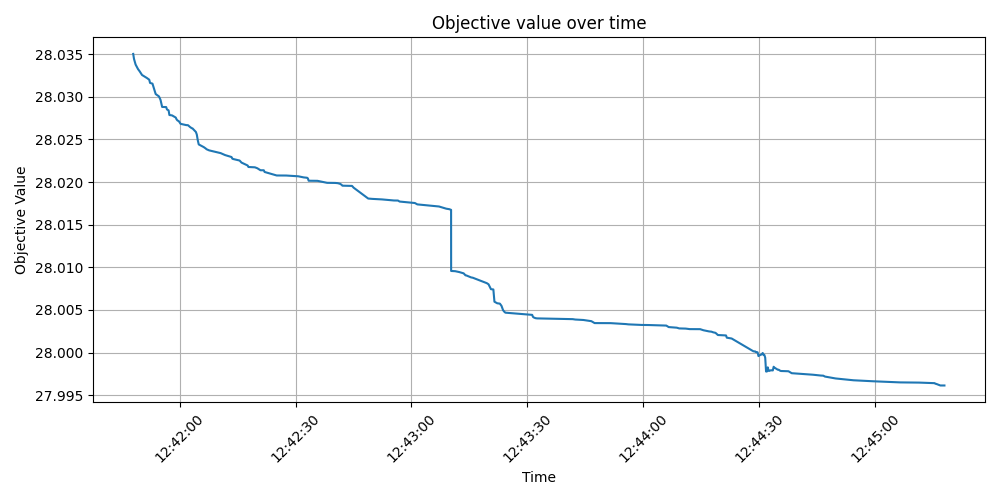
\includegraphics[width=1.0\textwidth]{figures/objective.png}
%% Use \caption command for figure caption and label.
\caption{Figure Caption}\label{fig:response-to-inclusion}
%% https://en.wikibooks.org/wiki/LaTeX/Importing_Graphics#Importing_external_graphics
\end{figure}

\subsection{Response to Exclusion}
\begin{figure}[H]%% placement specifier
%% Use \includegraphics command to insert graphic files. Place graphics files in 
%% working directory.
\centering%% For centre alignment of image.
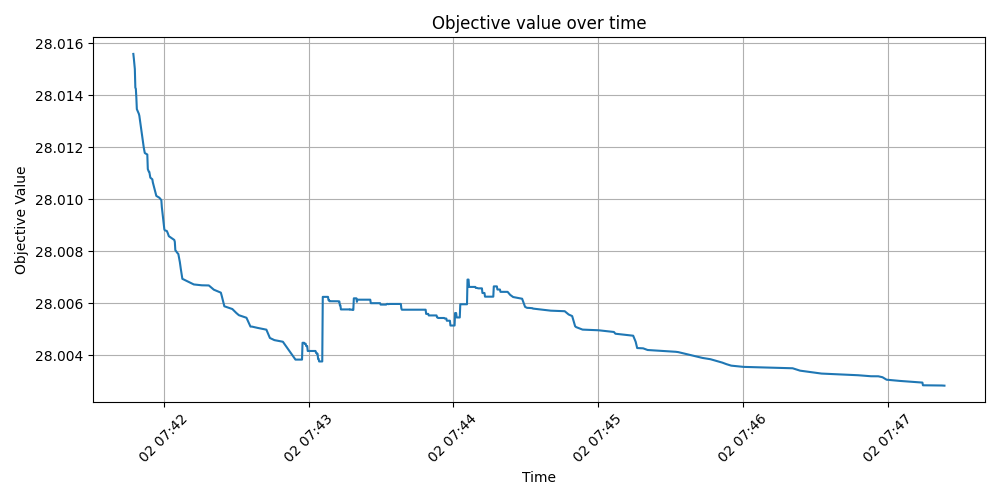
\includegraphics[width=1.0\textwidth]{figures/objective-400-exclusions.png}
%% Use \caption command for figure caption and label.
\caption{Figure Caption}\label{fig:objective-exclusion-400}
%% https://en.wikibooks.org/wiki/LaTeX/Importing_Graphics#Importing_external_graphics
\end{figure}

\subsection{Response to Changes in Knapsack Capacities}
The effects of changes to capacities will be illustrated in the same way as it was with the response to inclusion and below we see the table that shows which inputs that the ALNS will be affected by.

\begin{table}[H]
\centering
\begin{tabular}{|c|c|c|c|c|c|}
\hline
                      & \begin{tabular}[c]{@{}c@{}}At Time:\\ 01:00\end{tabular} & \begin{tabular}[c]{@{}c@{}}At Time:\\ 02:00\end{tabular} & \begin{tabular}[c]{@{}c@{}}At Time:\\ 03:00\end{tabular} & \begin{tabular}[c]{@{}c@{}}At Time:\\ 04:00\end{tabular} & \begin{tabular}[c]{@{}c@{}}At Time:\\ 05:00\end{tabular} \\ \hline
$\Delta |k|$ & 16                                                       & 16                                                       & 16                                                       & 16                                                       & 16                                                       \\ \hline
$\Delta |c|$ & 16                                                       & 16                                                       & 16                                                       & 16                                                       & 16                                                       \\ \hline
$\Delta |cap|$& 100                                                      & 200                                                      & 400                                                      & 800                                                      & 1600                                                     \\ \hline
\end{tabular}
\end{table}

\begin{figure}[H]%% placement specifier
%% Use \includegraphics command to insert graphic files. Place graphics files in 
%% working directory.
\centering%% For centre alignment of image.
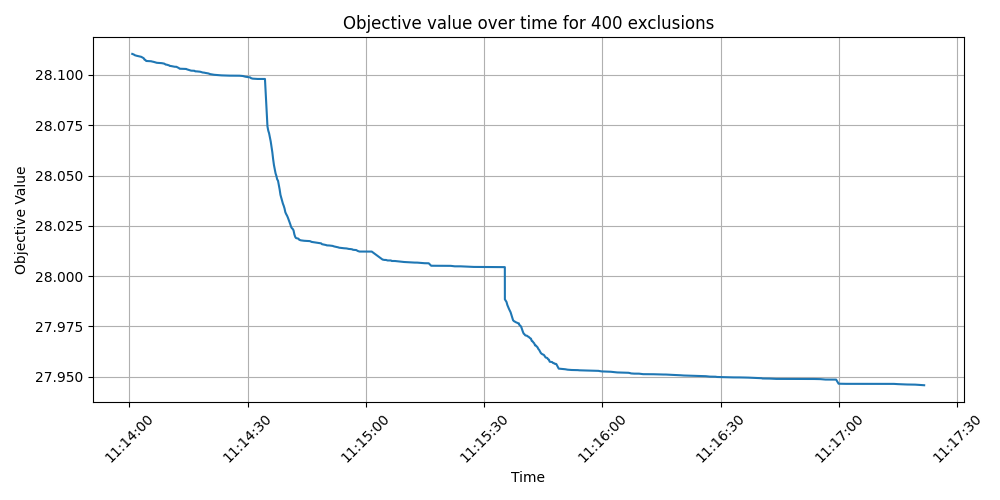
\includegraphics[width=1.0\textwidth]{figures/objective-resource-increases.png}
%% Use \caption command for figure caption and label.
\caption{Figure Caption}\label{fig:objective-resource-increases}
%% https://en.wikibooks.org/wiki/LaTeX/Importing_Graphics#Importing_external_graphics
\end{figure}

Correspondingly we also have the figure below in which the resources are decreasing.

\subsection{Response to Changes in Item Weights}
The final parameter that will be changed is the item set weights. This section will be more elaborate as we have to show how that the item sets are rearranged due to the changes in their weights across the different periods.

\begin{table}[H]
\centering
\begin{tabular}{|c|c|c|c|c|c|}
\hline
             & \begin{tabular}[c]{@{}c@{}}At Time:\\ 01:00\end{tabular} & \begin{tabular}[c]{@{}c@{}}At Time:\\ 02:00\end{tabular} & \begin{tabular}[c]{@{}c@{}}At Time:\\ 03:00\end{tabular} & \begin{tabular}[c]{@{}c@{}}At Time:\\ 04:00\end{tabular} & \begin{tabular}[c]{@{}c@{}}At Time:\\ 05:00\end{tabular} \\ \hline
$\Delta |i|$ & 20                                                       & 40                                                       & 80                                                       & 160                                                      & 320                                                      \\ \hline
$\Delta |k|$ & 26                                                       & 26                                                       & 26                                                       & 26                                                       & 26                                                       \\ \hline
$\Delta |v|$ & $1 \cdot 10^{5}$                                         & $2 \cdot 10^{5}$                                         & $4 \cdot 10^{5}$                                         & $8 \cdot 10^{5}$                                         & $1.6 \cdot 10^{6}$                                       \\ \hline
\end{tabular}
\end{table}

\section{Discussion}
\label{sec:4-discussion}
\subsection{Integration}
Figure \ref{fig:normal-setup}illustrates
a classic approach to operations research where a model allows the decision maker 
the obtain a solution to from which to make better informed decision. This approach is suitable to static problems and
problems there the parameters that make up the problem change slowly. This approach is often unsatisfactory in environments where
the environment is ever changing and the model parameters continually change in that light of new information. To solve this
problem a new field of dynamic and interactive metaheuristics show promise. 

Actor-based large neighborhood search enables tight integration between both the users and a 
dynamic data sources but crucially it naturally allows models to communicate with each other mimicking most 
practical decisions which are made up of multiple actors. For example, maintenance scheduling problems.

\begin{figure}[H]%% placement specifier
%% Use \includegraphics command to insert graphic files. Place graphics files in 
%% working directory.
\centering%% For centre alignment of image.
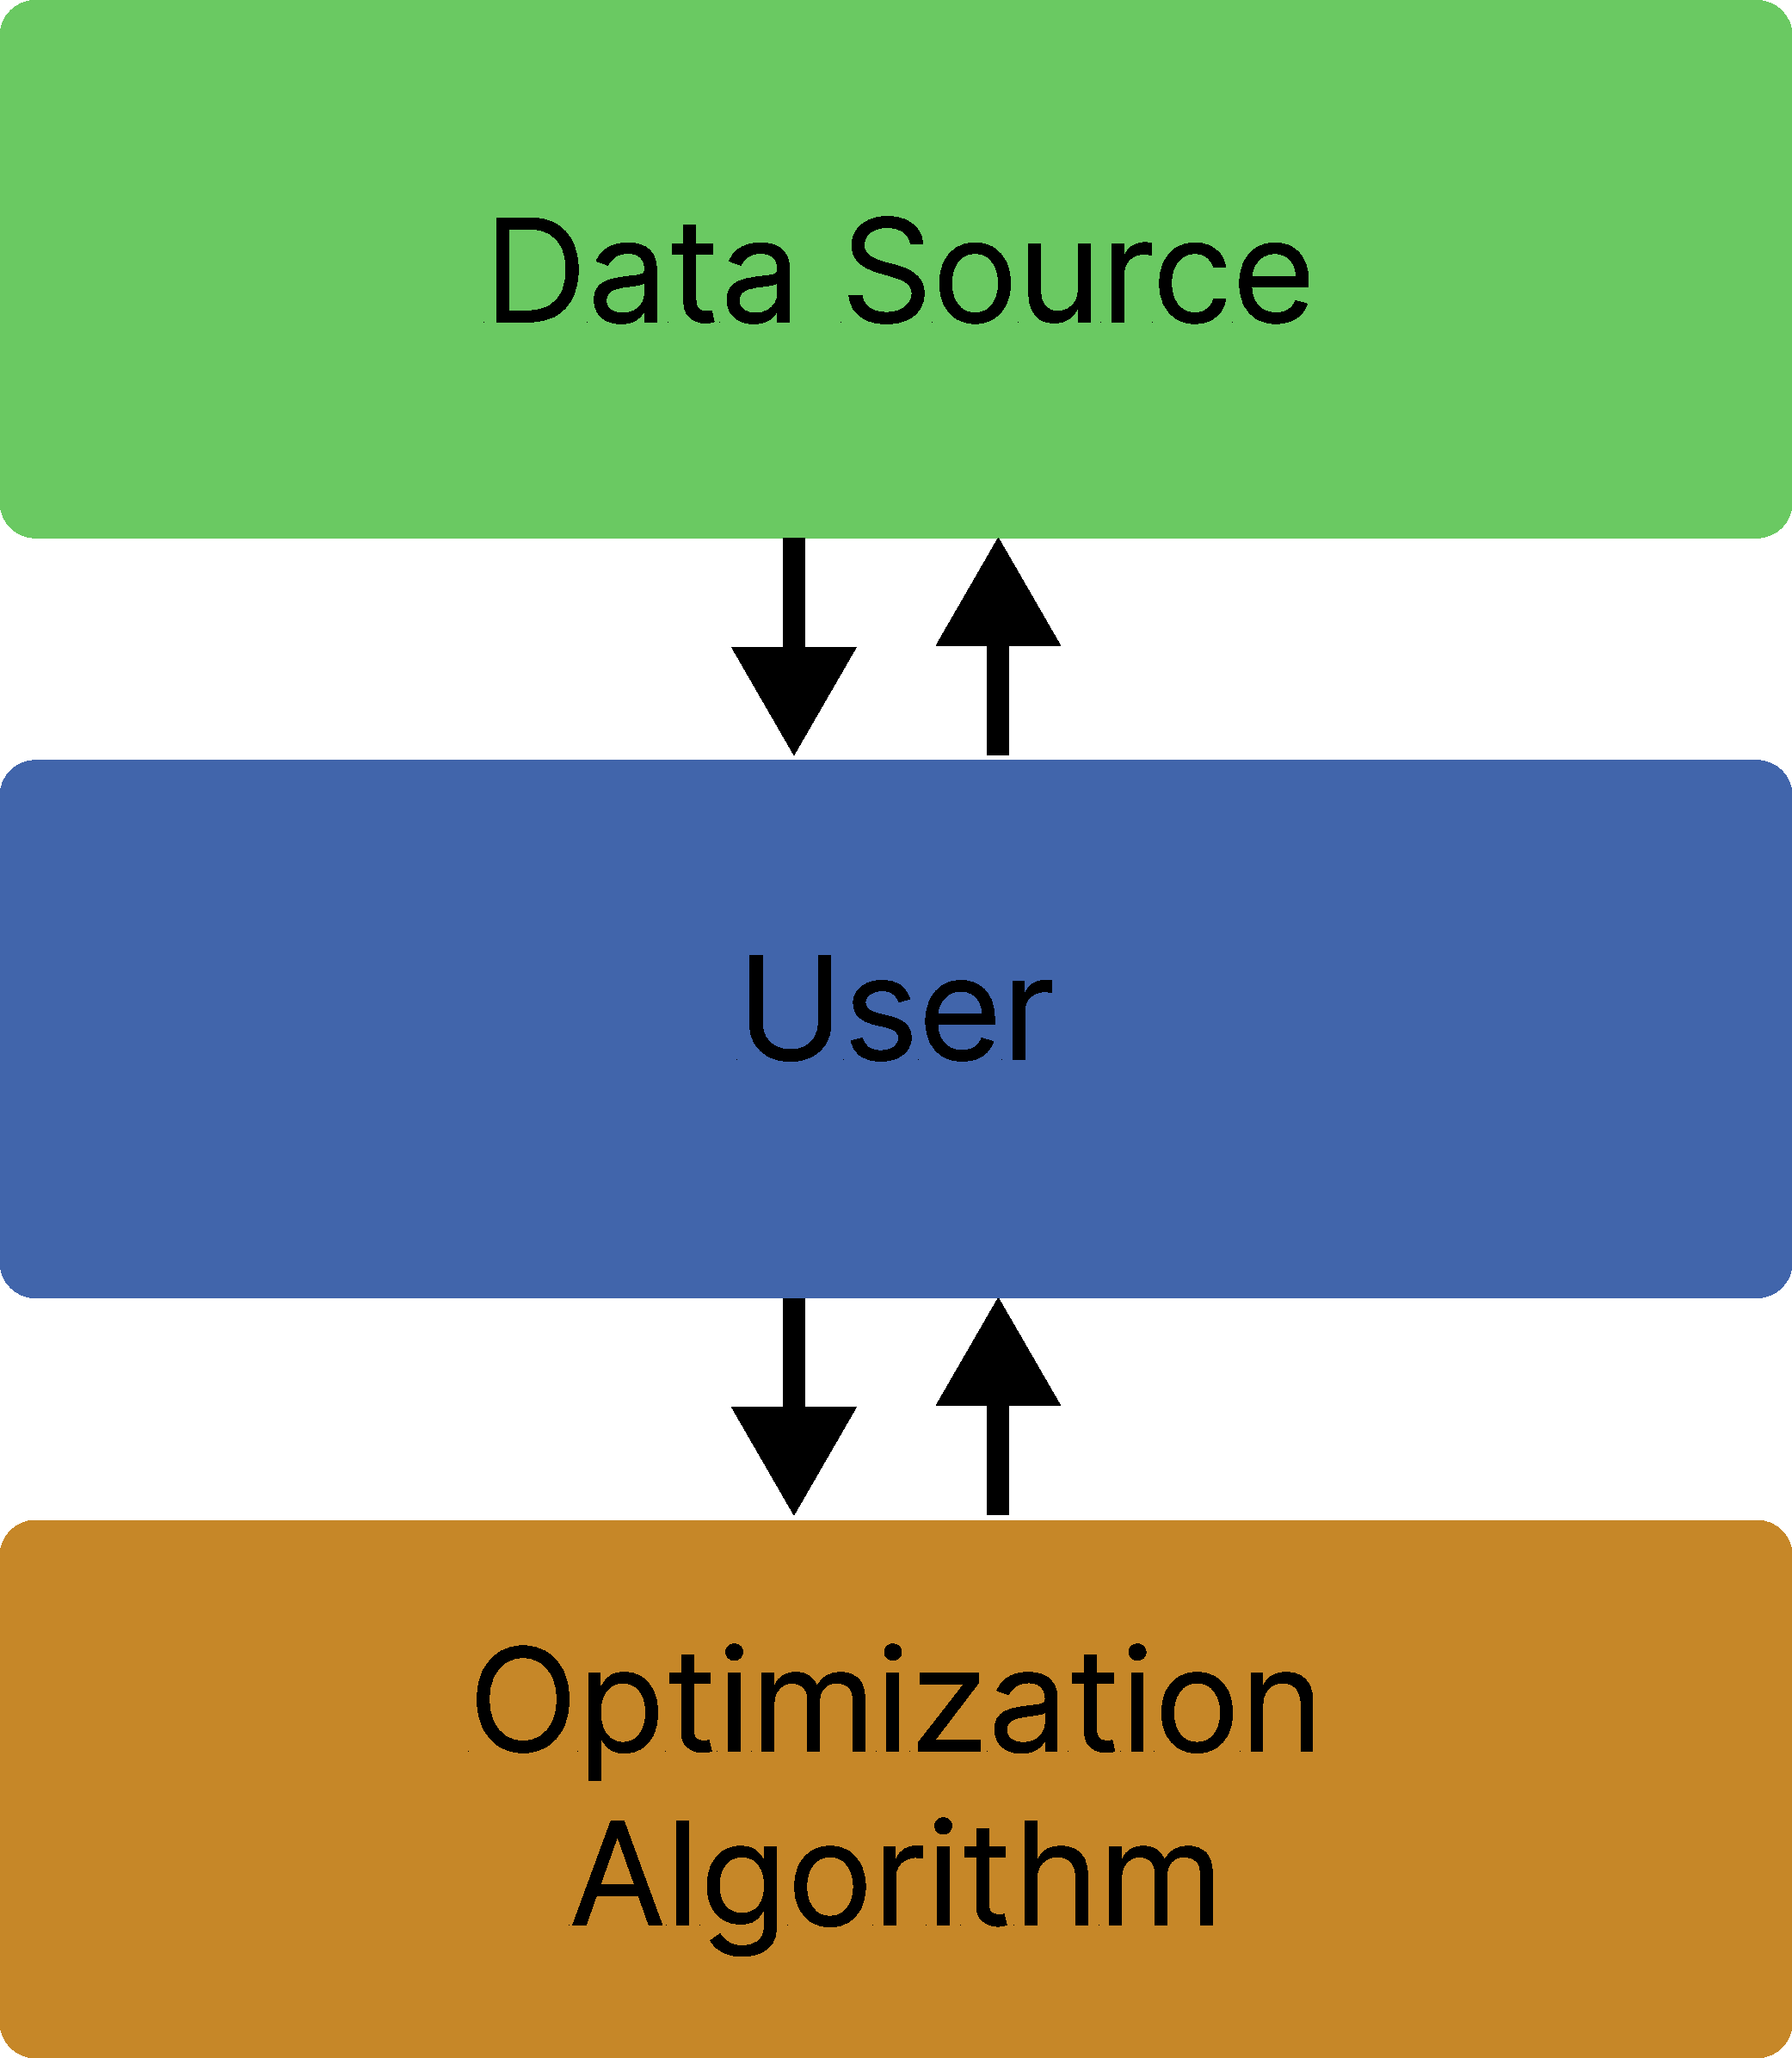
\includegraphics[width=0.2\textwidth]{figures/normal-setup.pdf}
%% Use \caption command for figure caption and label.
\caption{Traditional use case of developed optimization algorithms. Notice that the optimization algorithm is separated from the data source, requiring user interaction to optimize the process}
\label{fig:normal-setup}
%% https://en.wikibooks.org/wiki/LaTeX/Importing_Graphics#Importing_external_graphics
\end{figure}

Figure \ref{fig:actor-setup} illustrates the setup that is enabled by using an actor-based optimization approach. Due to the implemented message system it becomes possi 
\begin{figure}[H]%% placement specifier
%% Use \includegraphics command to insert graphic files. Place graphics files in 
%% working directory.
\centering%% For centre alignment of image.
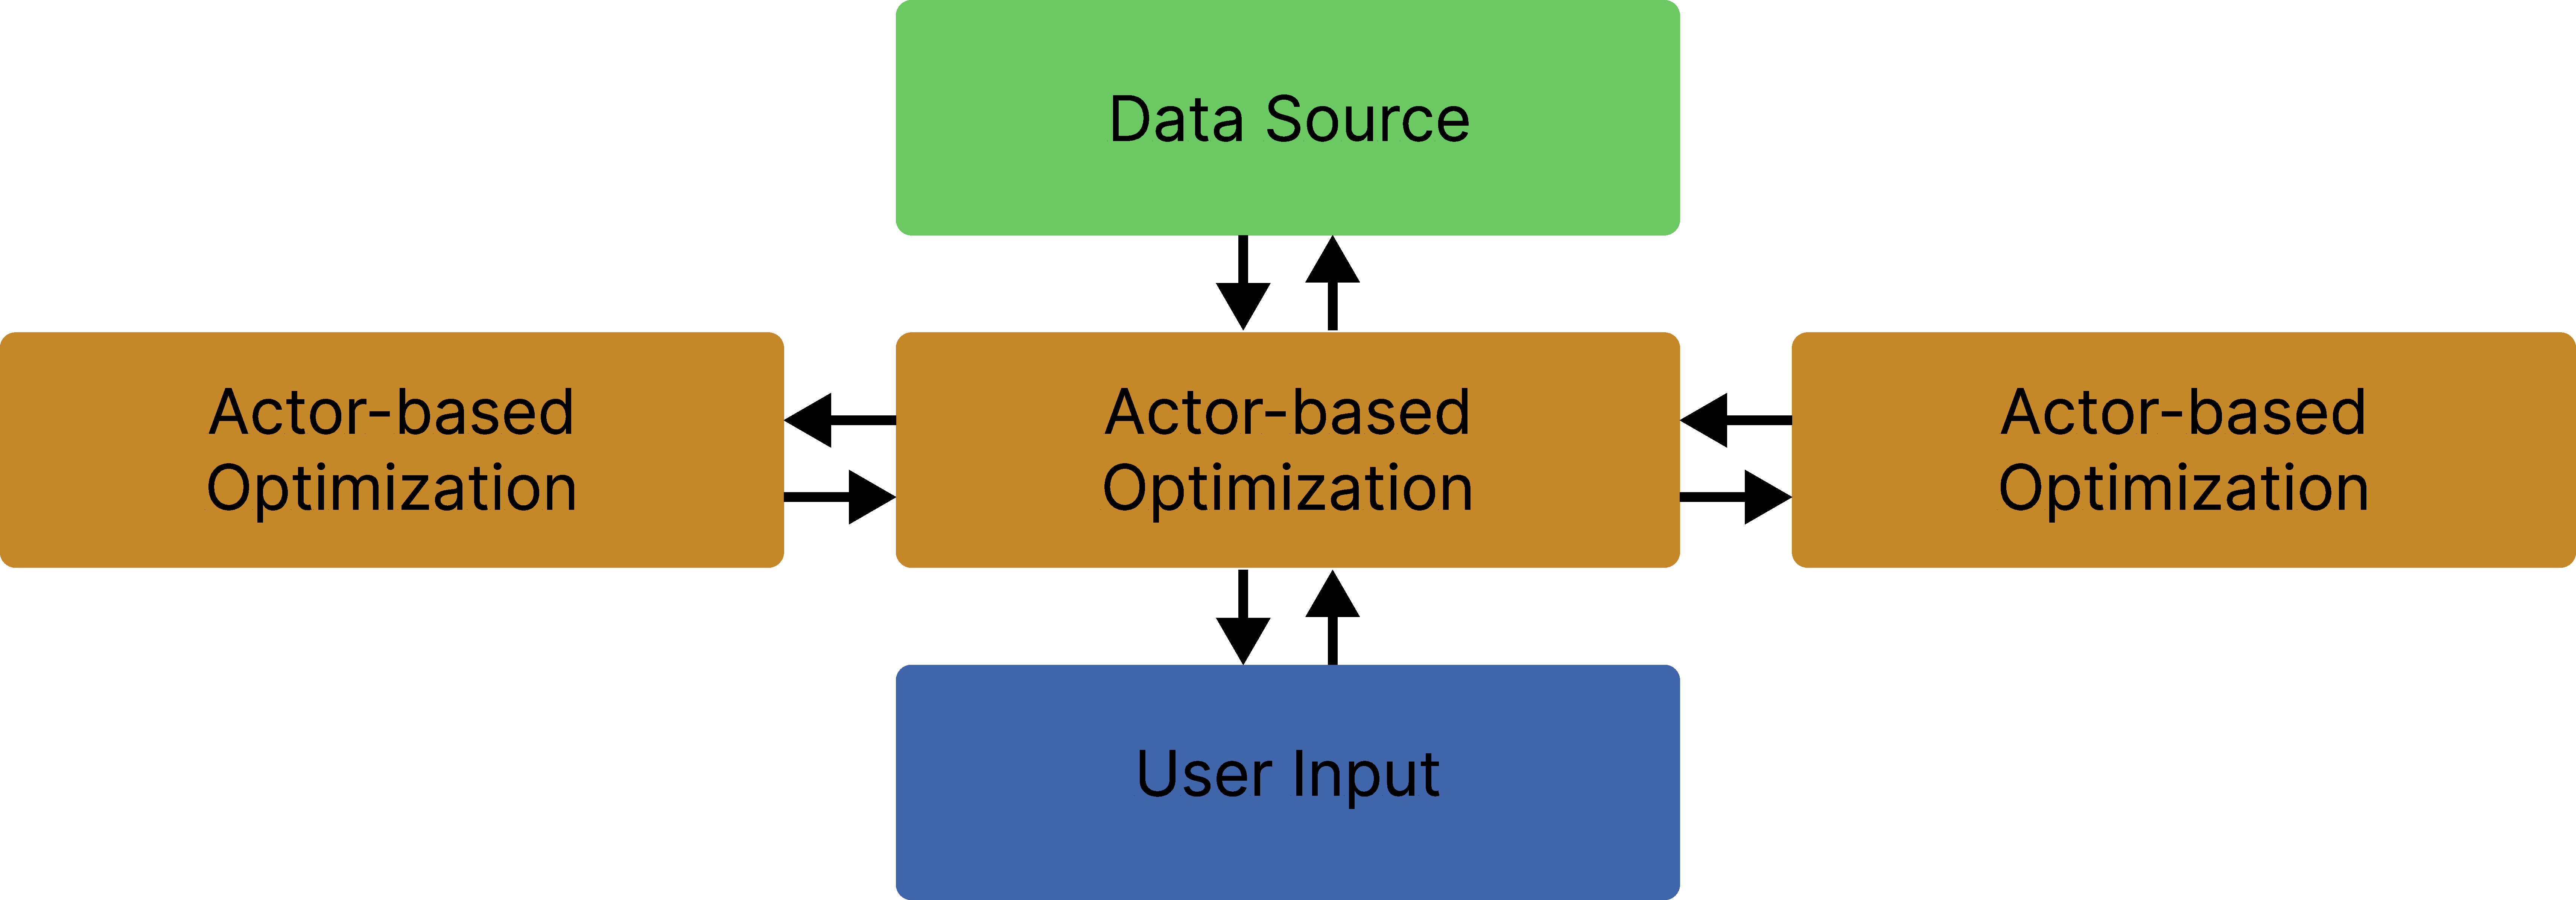
\includegraphics[width=0.65\textwidth]{figures/actor-setup.pdf}
%% Use \caption command for figure caption and label.
\caption{Figure Caption}\label{fig:actor-setup}
%% https://en.wikibooks.org/wiki/LaTeX/Importing_Graphics#Importing_external_graphics
\end{figure}

The three most conseqential properties of this approach is: 1. continual optimization saves the initial time it takes to reach converence significantly, 2. due to the message system the 
optimization approach will always be responsive to changes in both the parameter space
and the solution space, and 3. due to the encapsulation and message passing properties of the suggested optimization approach it becomes possible to apply the metaheuristic in multi-model 
and hierarchical model setups, providing an
approach for modelling and optimizing large scale systems. Finally a suggestion for future resarch directions will be given.

\subsection{Continuous Optimization}
By continually optimizing it becomes possible to only optimize the pertubations to the schedule. This means that we avoid having to optimize the problem to reach initial convergence.

In many cases this can save a significant amount of computations, refer to \cite{alza_bartlett_ceberio_mccall_2023}, especially if specilized constructors and destructors are implemented to handle the specific pertubations.

\subsection{Message Passing versus Restarts}
There is evidence that the effect of dynamic optimization is not always efficient, \cite{alza_bartlett_ceberio_mccall_2023} mentions the idea that dynamic optimization approaches can be "elusive" in that they do not always provide a speedup over restarting the solution method implementation. 
The paper clearly shows that dynamic approaches are the most effective when changes are small and frequent, which does align with the idea behind the actor-based LNS in that changes should be optimized around when ever they occur. T   


\subsection{System Level Optimization}
This approach could also enable larger scale optimzations providing a modular approach to operations research. This is beneficial 

%% Use \subsubsection, \paragraph, \subparagraph commands to 
%% start 3rd, 4th and 5th level sections.
%% Refer following link for more details.
%% https://en.wikibooks.org/wiki/LaTeX/Document_Structure#Sectioning_commands

%% Displayed equations can be tagged using various environments. 

%% Single line equations can be tagged using the equation environment.
%% Unnumbered equations are tagged using starred versions of the environment.
%% amsmath package needs to be loaded for the starred version of equation environment.
%% align or eqnarray environments can be used for multi line equations.
%% & is used to mark alignment points in equations.
%% \\ is used to end a row in a multiline equation.
%% Unnumbered versions of align and eqnarray

%% Refer following link for more details.
%% https://en.wikibooks.org/wiki/LaTeX/Mathematics
%% https://en.wikibooks.org/wiki/LaTeX/Advanced_Mathematics

%% Use a table environment to create tables.
%% Refer following link for more details.
%% https://en.wikibooks.org/wiki/LaTeX/Tables
% \begin{table}[t]%% placement specifier
% %% Use tabular environment to tag the tabular data.
% %% https://en.wikibooks.org/wiki/LaTeX/Tables#The_tabular_environment
% \centering%% For centre alignment of tabular.
% \begin{tabular}{l c r}%% Table column specifiers
% %% Tabular cells are separated by &
%   1 & 2 & 3 \\ %% A tabular row ends with \\
%   4 & 5 & 6 \\
%   7 & 8 & 9 \\
% \end{tabular}
% %% Use \caption command for table caption and label.
% \caption{Table Caption}\label{fig1}
% \end{table}


%% Use figure environment to create figures
%% Refer following link for more details.
%% https://en.wikibooks.org/wiki/LaTeX/Floats,_Figures_and_Captions
% \begin{figure}[t]%% placement specifier
% %% Use \includegraphics command to insert graphic files. Place graphics files in 
% %% working directory.
% \centering%% For centre alignment of image.
% \includegraphics{example-image-a}
% %% Use \caption command for figure caption and label.
% \caption{Figure Caption}\label{fig1}
% %% https://en.wikibooks.org/wiki/LaTeX/Importing_Graphics#Importing_external_graphics
% \end{figure}


%% The Appendices part is started with the command \appendix;
%% appendix sections are then done as normal sections
% \appendix
% \section{Example Appendix Section}
% \label{app1}

% Appendix text.

%% For citations use: 
%%       \citet{<label>} ==> Lamport (1994)
%%       \citep{<label>} ==> (Lamport, 1994)
%%
% Example citation, See \cite{interactive-optimization-methods} 
%% If you have bib database file and want bibtex to generate the
%% bibitems, please use
%%
%%  \bibliographystyle{elsarticle-harv} 
%%  \bibliography{<your bibdatabase>}

%% else use the following coding to input the bibitems directly in the
%% TeX file.

%% Refer following link for more details about bibliography and citations.
%% https://en.wikibooks.org/wiki/LaTeX/Bibliography_Management
\bibliography{/home/scipo/coding/papers/actor-based-large-neighborhood-search/bib/refs}

\bibliographystyle{elsarticle-harv}
\end{document}

\endinput
%%
%% End of file `elsarticle-template-harv.tex'.
